\documentclass[a4paper,12pt]{article}
\usepackage[english]{babel}
\usepackage[utf8]{inputenc}

% CSL style files for Mendeley and other referencing tools:
% https://github.com/citation-style-language/styles

%
% For alternative styles, see the biblatex manual:
% http://mirrors.ctan.org/macros/latex/contrib/biblatex/doc/biblatex.pdf
%
% The 'verbose' family of styles produces full citations in footnotes, 
% with and a variety of options for ibidem abbreviations.
%

\usepackage{graphicx}
\usepackage{csquotes}
\usepackage{amsfonts} % \mathbb in equations
\usepackage[style=verbose-ibid,backend=bibtex]{biblatex}

\usepackage[dvipsnames]{xcolor}

\usepackage{array}
\newcolumntype{L}{>{\centering\arraybackslash}m{3cm}}

\usepackage{algorithm}
\usepackage{algpseudocode}
\usepackage{caption}

\bibliography{sample}

\title{Markovian Approach to Positive-only Problems}

\author{Shayan Amani}

\begin{document}
\maketitle

%%%%%%%%%%%%%%%%%%%%%%%%%%%%%%%%%%%%%%%%%%%%%%%%%%%%%%%%%%%%%%%%%%%

\section{Preliminaries}

\subsection{Reinforcement Learning}
In reinforcement learning, the model trains from interactions with its environment (reward), instead of labeled data. Reinforcement learning falls in between \textit{supervised learning} and \textit{unsupervised learning} in which you have sparse (possibly) and time-delayed labels, so called \textit{rewards} 

\subsection{Action}

\subsubsection{Exploration vs. Exploitation dilemma}
Whether an AI should trust on the already learned part of the environment (exploitation) or trying new parts (actions, states, etc.) in hope for getting a higher \textit{reward} (exploration). 

\subsubsection{Credit assignment problem}
This issue discusses which of the previous actions had a major role in bringing the reward and how big it was the share of participation of that specific action in the reward.

\subsection{Reward}
Reward is nothing more than \textit{time-delayed} labels to help agent interact with the environment through trial and error. 
\subsubsection{Immediate and future reward}
Immediate reward, $r$ is what the agent gets after taking the action $a$ in state $s$ which leads to ending up in state $s'$. On the other side, we estimate immediate + future reward with $Q(s,a)$ function which is the total reward that taking action $a$ in state $s$ will fetch us in future.
\begin{equation}
    Q ^ { * } ( s , a ) = \mathbb { E } _ { s ^ { \prime } \sim \mathcal { E } } \left[ r + \gamma \max _ { a ^ { \prime } } Q ^ { * } \left( s ^ { \prime } , a ^ { \prime } \right) | s , a \right]
\end{equation}
we can call Q(s,a) is value of an action and V(s,a) function is value of a state. 

\subsection{Policy}
Number of possible policies is equal to number of actions to the power of the number of states.

\subsection{Prediction \& Control Tasks}
From the perspective of tasks, one can divide RL tasks into two distinct categories, prediction and control. It is worth to mention that policy iteration includes both prediction and control steps.

\subsubsection{Prediction}
We are given with the policy $\pi(a|s)$ and we need to \textit{predict} expected cumulative reward from any specified states. As an example of this task, we can mention \textbf{policy evaluation} step in algorithms such as Dynamic Programming.

\subsubsection{Control}
In this type of task we try to find a policy $\pi(a|s)$ which maximizes the expected cumulative reward. As an example of this task, we can mention \textbf{policy improvement} step in algorithms such as Dynamic Programming.

\subsection{On-policy vs. Off-policy}
Depending on how a method evaluates or improves the policy we can divide policies into two groups, on-policy and off-policy. In addition, there are two types of policy which need to be discussed here, behaviour and target policies. The policy that the algorithm uses to control the current action is behaviour and the policy that is being learned and/or evaluated is target

\subsubsection{On-policy methods}
This type of methods try to evaluate or improve the same policy from which the taken action comes. Examples of such methods are as follows:
\begin{itemize}
    \item Monte Carlo ES
    \item SARSA
\end{itemize}

\subsubsection{Off-policy methods}
These methods try to evaluate or improve a different policy than the one that used. Examples of such methods are as follows:
\begin{itemize}
    \item Q-learning
\end{itemize}

\subsection{Model-based vs. Model-free}
\textbf{Model-based} RL tries to enclose mechanics of the system. In that case, dependency on data for sampling would decrease. On the other hand, sampling is the major fact in \textbf{model-free} RL. Cost-wise talking, it is reasonable to probe a model instead of taking samples from a dataset or a simulator until sampling is not an expensive solution anymore. Unnecessary to mention that \textbf{transition probability P is the model} in model-based learning methods and has to be explicitly provided in such algorithms.

\subsubsection{General models}
The modeling frameworks can be used to represent the dynamics of the system are as follows:
\begin{itemize}
    \item Gaussian process: two similar inputs, yield two similar outputs too.
    \item Gaussian Mixture Model (GMM)
    \item Deep networks
\end{itemize}

\subsubsection{Model-based algorithms}
These group of algorithms completely dependent on transition probabilities which should be provided. List of a handful of such algorithms:
\begin{itemize}
    \item Dynamic programming
\end{itemize}

\subsubsection{Model-free algorithms}
Despite of previous category, these algorithms do not need transition probabilities and only rely on trial-and-error to probing their environment. List of a handful of such algorithms:
\begin{itemize}
    \item First-visit Monte Carlo
    \item TD-learning
    \item Q-learning
\end{itemize}

\subsection{Online vs. Batch RL}
\begin{itemize}
    \item Batch algorithms mostly occurred to be more stable.
    \item Data-wise speaking, batch algorithms can learn more efficient than online algorithms.
    \item Exploration is not possible when you use a batch algorithm.
\end{itemize}

\subsubsection{Online RL}
This type of learning picks an action and applies that drawn action to the environment and then observes the consequent state.

\subsubsection{Batch RL}
In this learning way, samples are extracted from the given dataset. We may have insufficient information about how and where the data are collected from.

%%%%%%%%%%%%%%%%%%%%%%%%%%%%%%%%%%%%%%%%%%%%%%%%%%%%%%%%%%%%%%%%%%%

\section{Bounding}
We can use available inequalities to bound our solution. We are always interested in finding upper bound for the policies or solution we propose. Hence, by applying those inequalities -based on requirements of each of them- the upper-bound can be found. Confidence intervals come into the problem where the results are bounded with an upper-bound. Moreover, confidence intervals are authentic measures of reliability of a solution.

\subsection{Martingales}
Sequence of random variable that:
\begin{equation}
    \mathbb { E } \left( X _ { n + 1 } | X _ { 1 } , \ldots , X _ { n } \right) = X _ { n }
\end{equation}

\subsection{Markov's inequality}
The most simplistic inequality among the other described here in terms of being relaxed about the constraints and requirements. The only requirement that needs to be satisfied is $X \geq 0$.
\begin{equation}
\mathbb {P}(X \geq a ) \leq \frac { \mathbb { E}( X ) } { a }
\end{equation}
Note that it should be not confused with Markov brothers' inequality.

\subsection{Chebyshev's inequality}
\begin{equation}
\mathbb {P}(|X - \mathbb{E}[X]| \geq a ) \leq \frac { \mathrm { Var}( X ) } { a^2 }
\end{equation}


\subsection{Hoeffding's inequality}
Using Hoeffding's lemma we can prove this inequality which the definition is as follows:

Let $X_i$ be a bounded random variable with $X_i \in [b, d]$:
\begin{equation}
    \mathbb {P} \left( \left| \frac{1}{n} \sum_{i=1}^{n} X_i - \mathbb{E}[X_i] \right| \geq a \right) \leq { \exp \left( \frac{-2 n a ^ {2} }{ \left(d-b \right) ^ 2} \right) }
\end{equation}

In order to prove the above inequality we need to use Hoeffding's lemma:
\begin{equation}
    \mathbb {E} \left[ \exp \left( {\lambda ( X - \mathbb {E}[X] )} \right)  \right] \leq \exp \left( \frac{\lambda ^ 2 (d-b)^2}{8} \right)
\end{equation}

As PAC Optimal MDP Planning paper \autocite{Telghan et al. 2015} proposed they replaced Hoeffding-bound with Weissman confidence interval.

\subsection{Bernstein inequalities}
\begin{equation}
    \mathbb { P } \left( \left| \frac { 1 } { n } \sum _ { i = 1 } ^ { n } X _ { i } \right| > a \right) \leq 2 \exp \left( \frac {- n a ^ {2} } { 2 \left( 1 + \frac {a} {3} \right) } \right)
\end{equation}

%%%%%%%%%%%%%%%%%%%%%%%%%%%%%%%%%%%%%%%%%%%%%%%%%%%%%%%%%%%%%%%%%%%

\section{Methodologies}
We are studying a simulator-based MDP problem. transition probabilities and rewards can be generated by the simulator which is a generative model built upon different environmental parameters.

\subsection{LSPI}
Finds and learns a linear approximation of Q-function. LSPI is a generalization of LSTDQ. This algorithm never diverges or return meaningless answers.

\begin{itemize}
    \item Model-free algorithm
    \item Batch RL algorithm
    \item As a downside it ignores the exploration problem.
\end{itemize}

\subsection{First-visit Monte Carlo}
For building a model using repeated \textbf{random sampling} \autocite{For more read on Thompson sampling}. It works only on episodic tasks. Because FVMC updates all the action's value based on the final return, it has no bias at all.
\begin{itemize}
    \item model-free
    \item episodic
    \item  all steps look ahead (observes rewards for \textbf{all steps} in an episode)
    \item higher variance than TD: W $\leftarrow$ W $\frac{1}{b(A|S)}$ b is probability and if it becomes very small so W becomes so big.
    \item no bias
\end{itemize}

\subsection{TD(0)}
TD-learning has lower \textit{variance} (than FVMC) because it depends on less factors. This algorithm only updates previous action's value based on the current action's value. TD captures recent trends. TD has some bias (again compared to FVMC) as values are updated towards the prediction.
\begin{itemize}
    \item model-based
    \item one step look ahead
    \item lower variance
    \item some biases
\end{itemize}

\subsection{Q-learning}
A variation of TD-learning which calculates and (then iteratively updates) Q function -which represents (predicts) maximum cumulative discounted reward with performing action $a$ in state $s$- using Bellman equation. This method is a table-based (tabular) algorithm and we use Q-table as a table with the dimensions of states $\times$ actions.

\subsection{$\epsilon$-greedy}
Popular in Deep Reinforcement Learning (DRL) which makes a good trade-off in terms of exploration and exploitation.

\subsection{Deep Reinforcement Learning}
Intrinsic to supervised learning methods, training is always time consuming and from a specific stage and on it becomes little-to-no improvement so the reasonable choice is switching to Reinforcement Learning framework.

\subsubsection{Deep Q-Network (DQN)}
Renowned for solving higher dimensional problems like Atari games. All of the steps are explained in Algorithm~\ref{alg:DQN}.

\begin{itemize}
    \item batch RL algorithm
\end{itemize}

\begin{algorithm}[H]
\caption{DQN algorithm in batch mode}
\label{alg:DQN}
\begin{algorithmic}[1]
    \State Init D \Comment{\textcolor{BlueViolet}{replay memory}}
    \State Init Q \Comment{\textcolor{BlueViolet}{Q-table w/ random weights}}
    \State \textcolor{OrangeRed}{Get} or Observe $s_0$ \Comment{\textcolor{BlueViolet}{the initial state}}
    \For{each episode}
        \For{samples in each episode}
            \State \textit{\textcolor{OrangeRed}{- skip $\epsilon$-greedy exploration}}
            \State $a = argmax_a Q(s,a)$
            \State \textit{\textcolor{OrangeRed}{- skip applying action $a$ to the environment}}
            \rlap{\smash{$\left.\begin{array}{@{}c@{}}\\{}\\{}\end{array}\color{BlueViolet}\right\}%
              \color{BlueViolet} experience$}}
            \State \textcolor{OrangeRed}{Get} or Observe $r, s'$
            \State Store the \textbf{experience} $<s, a, r, s'>$ in replay memory $D$
            \State \textit{Random} \textbf{sampling} from $D$ $<ss, aa, rr, ss'>$  \Comment{\textcolor{BlueViolet}{[mini]-batch}}
            \If{$ss' \neq $ terminal state} \Comment{\textcolor{BlueViolet}{target for each mini-batch}}
                \State $tt = rr + \gamma max_{aa'} Q(ss', aa')$
            \Else
                \State $tt = rr$
            \EndIf
            \State Train the network
        \EndFor    
    \EndFor
\end{algorithmic}
\end{algorithm}

% \algnewcommand{\algorithmicgoto}{\textbf{go to}}%
% \algnewcommand{\Goto}[1]{\algorithmicgoto~\ref{#1}}%
% \begin{algorithm}
%   \caption{Euclid’s algorithm}\label{euclid}
%   \begin{algorithmic}[1]
%     \Procedure{Euclid}{$a,b$}\Comment{The g.c.d. of a and b}
%     \State $r\gets a\bmod b$
%     \While{$r\not=0$} \Comment{We have the answer if r is 0}\label{marker}
%       \State $a\gets b$
%       \State $b\gets r$\hspace*{4em}%
%         \rlap{\smash{$\left.\begin{array}{@{}c@{}}\\{}\\{}\\{}\\{}\end{array}\color{red}\right\}%
%           \color{red}\begin{tabular}{l}We loop here\\until $r=0$.\end{tabular}$}}
%       \State $r\gets a\bmod b$
%     \EndWhile
%     \State \textbf{return} $b$\Comment{The gcd is b}
%     \State \Goto{marker}
%   \EndProcedure
% \end{algorithmic}
% \end{algorithm}


\subsubsection{Experience Replay}
DQN mostly Relied on a stabilization technique with neural networks, called Experience replay.



\subsubsection{Deep Deterministic Policy Gradient (DDPG)}
Good choice for continuous action space such as real-world control tasks.

\begin{table}
    \centering
    \begin{tabular}{|c|L|L|L|L|}
        \hline
        \textbf{Method}  &    \textbf{Model Dependence}    &   \textbf{Policy Dependence}   &   \textbf{Action Continuity}  & \textbf{Parent Algorithm(s)}\\
        \hline
        \hline
        DQN &   model-free  &   on-policy   &   discrete    &   Q-learning, DL\\
        \hline
        DDPG    &   model-free  &   on-policy   &   continuous  &   Actor-critic\\
        \hline
    \end{tabular}
    \caption{DRL methods comparison chart}
    \label{tab:my_label}
\end{table}

%%%%%%%%%%%%%%%%%%%%%%%%%%%%%%%%%%%%%%%%%%%%%%%%%%%%%%%%%%%%%%%%%%%

\section{Bayesian Settings}
Sampling using a logistic regression (or any other methods) we can generate some distributions for our features (bio10 and bio5 REVIEW and alpha) then we are able to feed these to a linear program to calculate weights (L1 norm or any other distance metrics) and then we can build our ambiguity set based on what we get as weights.
\subsection{Dirichlet Distribution}
    In Bayesian analysis, this type of distribution is widely used as prior distribution.
    
\subsection{Pareto Distribution}
    People usually use this distribution as a tool to model the tail region of another distribution.
% 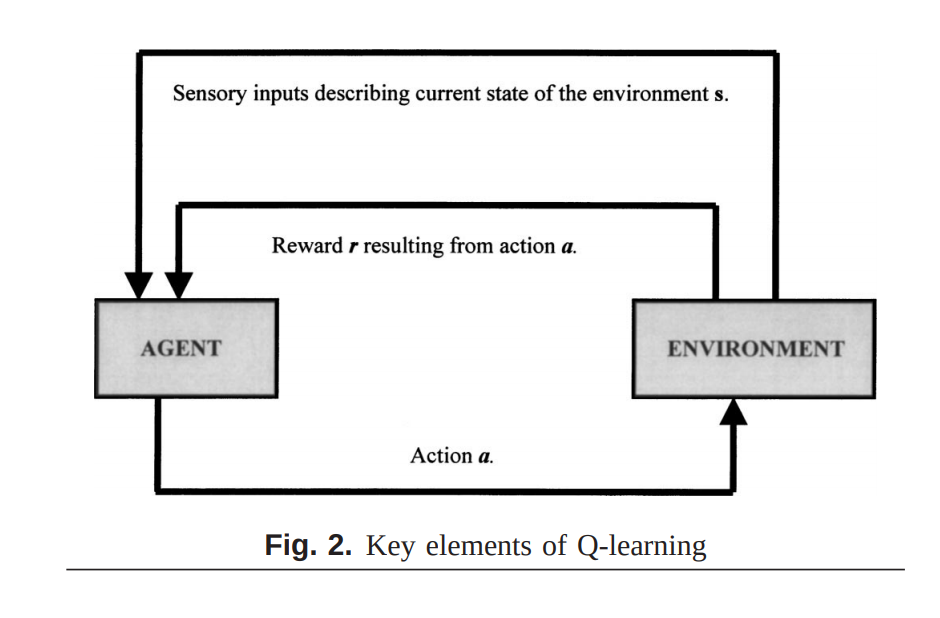
\includegraphics[width=1\columnwidth]{elements.png}

%%%%%%%%%%%%%%%%%%%%%%%%%%%%%%%%%%%%%%%%%%%%%%%%%%%%%%%%%%%%%%%%%%%

\section{Multi-armed Bandit Problem vs. A/B Test}
In a multi-armed bandit problem agent choose and pull one of the arms randomly at the beginning. The pulled arm bandit generates a distribution with specific values of mean $\mu_i$ and variance. The distribution is stationary but still unknown before pulling. \autocite{Strehl and Littman 2008}

\begin{tabular}{|c|c|}
    \hline
    \textbf{A/B test}    &   \textbf{Multi-armed bandit}  \\
    \hline
    \hline
    pure exploration    &   exploration along with exploitation \\
    \hline
    return after completion &   immediate return while running \\
    \hline
    expensive   &   cost-efficient \\
    \hline
\end{tabular}

\subsubsection{Upper Confidence Bound Algorithm}
Upper confidence interval includes true expected value and it gets narrow down (becomes smaller) after each iteration of the algorithm. In other words, the agent becomes more assured about the return value as it runs through each iterations. The agent picks the next upper confidence interval to exploit and continue with that until it finds a new higher value. Unneeded to mention that the two main actor in this algorithm are as follows:
\begin{itemize}
    \item Confidence interval becomes tighter along with iterations
    \item Return value along iterations converges to the expected true value.
\end{itemize}

%%%%%%%%%%%%%%%%%%%%%%%%%%%%%%%%%%%%%%%%%%%%%%%%%%%%%%%%%%%%%%%%%%%

\section{Paper Summaries}

\subsection{Deep Q-Learning}


%%%%%%%%%%%%%%%%%%%%%%%%%%%%%%%%%%%%%%%%%%%%%%%%%%%%%%%%%%%%%%%%%%%

\section{Case Study}
The current case is a study on an invasive plant (non-native to the ecosystem) in New England area, namely glossy buckthorn [capitalization?].

%%%%%%%%%%%%%%%%%%%%%%%%%%%%%%%%%%%%%%%%%%%%%%%%%%%%%%%%%%%%%%%%%%%

\section {Future Review}
\begin{itemize}
    \item Interval Estimation approach relationship with multi-armed bandit.
    \item Thompson sampling
    \item Bernstein inequalities
    \item DRL approach to invasive species management
\end{itemize}


% This is an example citation \autocite{ginsberg}.
% \lipsum[1] % dummy text

% This is another example citation \autocite{brassard}.
% \lipsum[2] % dummy text

% This is a repeated citation \autocite{brassard}.
% \lipsum[3] % dummy text

% This is another example citation \autocite{adorf}.
% \lipsum[4] % dummy text 

\end{document}